\documentclass[letterpaper, 12pt]{report}
\usepackage[utf8]{inputenc}
\usepackage[english, spanish]{babel}
\usepackage{fullpage} 
\usepackage{graphicx}
\usepackage{enumitem}
\usepackage{chngcntr}
\usepackage{float}
\usepackage{hyperref} 
\counterwithin{figure}{section}
\renewcommand{\thesection}{\arabic{section}}
\renewcommand{\thesubsection}{\thesection.\arabic{subsection}}
\renewcommand{\baselinestretch}{1.5}
\begin{document}

\begin{titlepage}
	\centering
	
\includegraphics[width=0.3\textwidth]{eii_ulpgc.png}\par\vspace{1cm}
	{\scshape\LARGE Universidad de Las Palmas de Gran Canaria \par}
	\vspace{1cm}
	{\scshape\Large Programaci\'on de Aplicaciones M\'oviles Nativas \par}
	\vspace{.2cm}
    {\scshape\Large Diseño de interfaces. \par}
	\vspace{1cm}
	{\Large\bfseries Documento de Diseño para la Aplicación QRseekers\par}
	\vspace{1cm}
	{\itshape Paula Rosa Rodríguez Morales y Anna Sajdokova \par}
	\vfill

	\vfill
	{\large \today\par}
\end{titlepage}
\tableofcontents
\newpage

\section{Introducción}
El presente documento de diseño para la aplicación QRseekers: The City Discovery Game se centra en describir de manera detallada los aspectos clave del diseño de la aplicación, sus funcionalidades principales y los mockups que ilustran la experiencia de usuario. QRseekers está concebida como una herramienta interactiva que utiliza la gamificación para transformar la exploración de ciudades en una actividad competitiva y educativa. A través del uso de códigos QR y preguntas relacionadas con puntos de interés locales, los usuarios pueden aprender mientras avanzan en el juego.

En este trabajo se abordarán tanto los objetivos y características fundamentales de la aplicación como el diseño de sus interfaces, desde la pantalla de inicio hasta el sistema de clasificaciones en tiempo real. Además, se incluirán los mockups que ilustran cada una de las pantallas clave, permitiendo visualizar el flujo de interacción y la usabilidad de QRseekers. Este análisis detallado ofrece una visión integral del proceso de diseño y desarrollo de la aplicación, destacando su enfoque intuitivo, flexible y adaptable para diferentes ciudades y usuarios.

\newpage

\section{Resumen de la aplicación}

QRseekers es una aplicación móvil creada para transformar la manera en que las personas exploran y descubren ciudades. Su diseño está centrado en ofrecer una experiencia interactiva y educativa, que permite a los usuarios conocer los puntos más emblemáticos de una ciudad mientras participan en un juego competitivo basado en la búsqueda de códigos QR. Estos códigos, escondidos en ubicaciones estratégicas cerca de monumentos y lugares de interés, no solo ofrecen una manera entretenida de moverse por la ciudad, sino que también desencadenan preguntas relacionadas con la historia, la cultura y la geografía locales, incentivando el aprendizaje en cada paso del recorrido.

El concepto clave detrás de QRseekers es el uso de códigos QR como una puerta de acceso a contenido educativo. Los jugadores deben buscar y escanear estos códigos para desbloquear una serie de preguntas en cada ubicación. El juego plantea dos tipos de preguntas: una obligatoria, que es necesaria para avanzar al siguiente punto del recorrido, y preguntas opcionales que ofrecen puntos adicionales. Estas preguntas varían en formato, ya que pueden ser de opción múltiple, respuestas numéricas o de texto. Además, el juego introduce una dinámica especial llamada "Catch the Golden Pig", en la que los jugadores tienen que localizar a una persona específica dentro de la ciudad para obtener una contraseña y resolver una pregunta abierta, añadiendo un elemento de sorpresa y emoción a la experiencia.

\newpage

\section{Objetivos de la app}
Los principales objetivos de la aplicación QRseekers son:
\begin{itemize}
    \item Promover la exploración de ciudades: Facilitar que los usuarios descubran puntos turísticos e históricos.
    \item Fomentar el aprendizaje interactivo: Enseñar sobre la historia y la cultura local mediante preguntas asociadas a los lugares visitados.
    \item Impulsar la competencia sana: Proporcionar un entorno competitivo y divertido mediante el sistema de puntos y clasificaciones.
    \item Ofrecer flexibilidad y escalabilidad: Permitir la personalización de la aplicación para múltiples ciudades, juegos y eventos.
\end{itemize}

\newpage

\section{Funcionalidades clave}
Uno de los aspectos más atractivos de QRseekers es su modo de juego en equipo. Los usuarios pueden formar equipos donde un miembro será responsable de responder las preguntas, pero los puntos se distribuyen equitativamente entre todos. Esto permite que cada equipo avance de manera conjunta y refuerza la cooperación y el trabajo en grupo. A lo largo del juego, las clasificaciones de los equipos se muestran en tiempo real en una tabla de posiciones, lo que añade una sana competencia entre los participantes. Al final de cada recorrido, la tabla se congela momentáneamente para anunciar al equipo ganador, brindando una sensación de anticipación y cierre emocionante.

La aplicación también destaca por su flexibilidad y escalabilidad, permitiendo su uso en múltiples ciudades. QRseekers no es una experiencia única para una sola ciudad, sino que está diseñada para adaptarse fácilmente a cualquier lugar del mundo. Esto se logra mediante la carga de nuevos conjuntos de códigos QR y preguntas específicas para cada ubicación, lo que permite a los creadores de contenido o socios locales personalizar la experiencia según las particularidades de su región. Cada juego es único y puede descargarse previamente para jugar sin conexión, lo que garantiza que los usuarios puedan disfrutar de la experiencia incluso en lugares con cobertura de internet limitada.

Además de los jugadores, la aplicación cuenta con un sistema de administración robusto que permite a los administradores controlar diversos aspectos del juego. Estos pueden crear y cerrar juegos, modificar equipos y actualizar el contenido en tiempo real. Este nivel de gestión es clave para la organización de eventos o juegos temáticos, donde las instituciones locales, gobiernos o empresas turísticas pueden diseñar experiencias específicas para sus usuarios.

\newpage

\section{Detalles técnicos}
En términos técnicos, la aplicación está disponible para dispositivos Android. Además, el backend de la aplicación almacena toda la información necesaria para gestionar los juegos: las ubicaciones de los códigos QR, las bases de datos de preguntas y respuestas, así como las puntuaciones de los jugadores y equipos. Para garantizar la seguridad y evitar trampas, los códigos QR estarán vinculados a coordenadas GPS específicas, lo que significa que solo pueden ser escaneados cuando los jugadores se encuentren en la ubicación correcta.

\newpage

\section{Wireframes de la aplicación móvil}
A continuación, se mostrarán los wireframes de la aplicación móvil de QRseekers, donde se verán las pantallas principales que guían la experiencia del usuario desde el inicio hasta la selección de un juego. Aquí están los aspectos principales de cada una de las pantallas:

\subsection{Pantalla de inicio}

\begin{itemize}
    \item Diseño y mensaje: Presenta un diseño limpio y atractivo que incluye el logo de QRseekers y una ilustración de dos personajes explorando un mapa, lo cual refuerza la idea de una experiencia de descubrimiento y juego colaborativo.
    \item Texto promocional: El eslogan 'Explore the city with friends' invita a los usuarios a comenzar una aventura divertida con amigos, resaltando el enfoque social de la aplicación.
\end{itemize}

\begin{figure}[H]
\centering
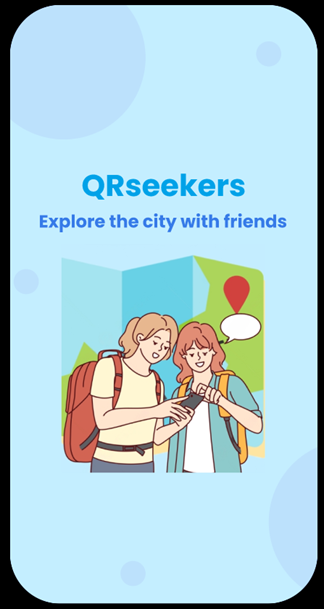
\includegraphics[width=0.4\textwidth]{figure1.png}
\caption{Landing screen.}
\label{fig:1}
\end{figure}

\subsection{Pantalla de registro}

\begin{itemize}
    \item Formulario de registro: Esta pantalla incluye un formulario simple para que los usuarios ingresen sus datos y se registren en la aplicación. Se solicitan: nombre, correo electrónico, nombre de usuario, contraseña (con un campo adicional para confirmarla), botón de registro
    \item Acuerdo de privacidad: Hay una casilla que los usuarios deben marcar, confirmando que aceptan que sus datos serán procesados y almacenados por QRseekers, y que las fotos durante la actividad podrían ser usadas en redes sociales. Este es un detalle importante desde el punto de vista legal y de privacidad.
\end{itemize}

\begin{figure}[H]
\centering
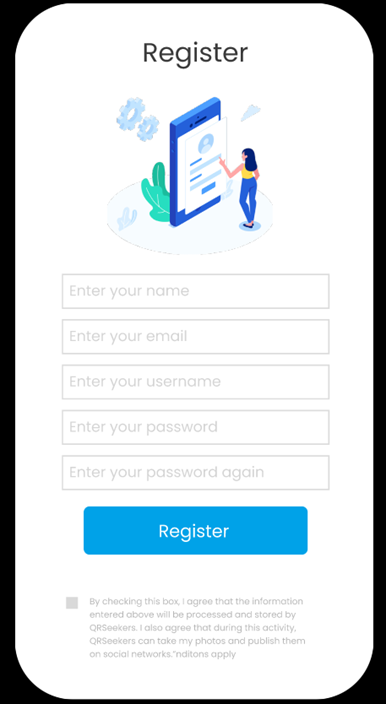
\includegraphics[width=0.4\textwidth]{figure2.png}
\caption{Register screen.}
\label{fig:1}
\end{figure}

\subsection{Pantalla de inicio de sesión}

\begin{itemize}
    \item Formulario de inicio de sesión: Similar a la pantalla de registro, se presentan campos para que el usuario ingrese su nombre de usuario y contraseña.
    \item Botón de Inicio de Sesión: Un botón claro y destacado que dice 'Login' para acceder a la aplicación.
    \item Opciones de recuperación: Se incluye un enlace 'Forgot your password?' para aquellos usuarios que necesiten recuperar su contraseña, además de un mensaje que dirige a los usuarios que no están registrados a hacerlo con el texto: 'Not registered yet? Sign up now!'
\end{itemize}

\begin{figure}[H]
\centering
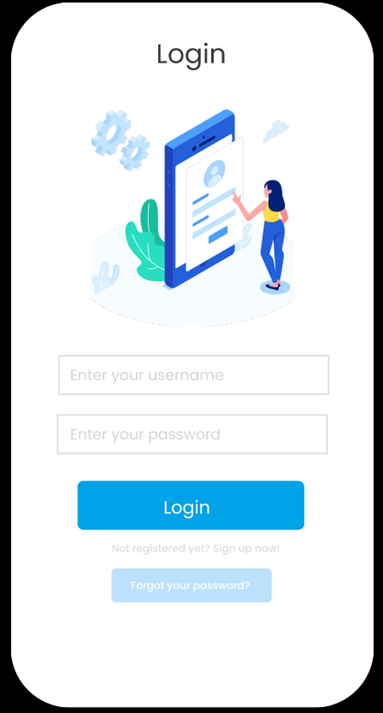
\includegraphics[width=0.4\textwidth]{figure3.png}
\caption{Login screen.}
\label{fig:1}
\end{figure}

\subsection{Pantalla de selección de juego}

\begin{itemize}
    \item Lista de juegos disponibles: En esta pantalla, el usuario puede seleccionar entre distintos juegos disponibles. Los juegos se presentan en tarjetas con colores diferenciados y descripciones breves que indican el tipo de experiencia que ofrece cada uno. 
    \item Botón de confirmación: Después de seleccionar el juego deseado, hay un botón de 'Submit your selection' para confirmar y proceder.
\end{itemize}

\begin{figure}[H]
\centering
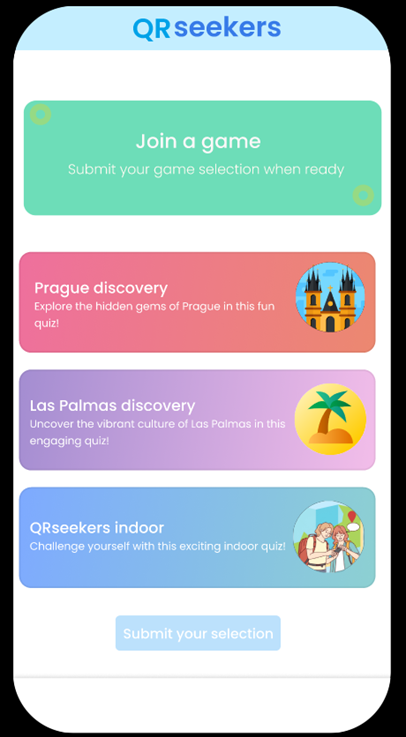
\includegraphics[width=0.4\textwidth]{figure4.png}
\caption{Game selection screen.}
\label{fig:1}
\end{figure}

\subsection{Pantalla de asignación de equipo}

\begin{itemize}
    \item Mensaje de espera: En esta pantalla, se indica a los usuarios que esperen mientras se realiza la asignación de equipos.
    \item Reglas del juego: Se despliegan las reglas principales.
\end{itemize}

\begin{figure}[H]
\centering
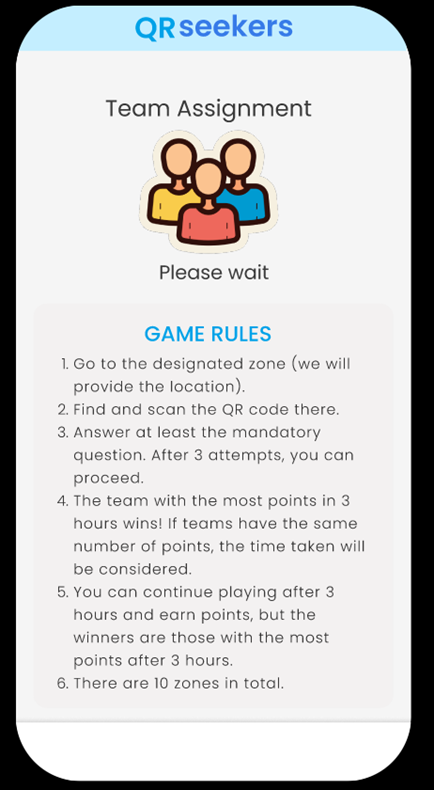
\includegraphics[width=0.4\textwidth]{figure5.png}
\caption{Team assignment screen.}
\label{fig:1}
\end{figure}

\subsection{Pantalla del equipo}

\begin{itemize}
    \item Nombre del equipo: En esta captura, se muestra al usuario el nombre de su equipo, en este caso 'The Garlic Gurus'.
    \item Identificación del equipo: Los nombres de los miembros del equipo aparecen enumerados para que los jugadores puedan ubicarse entre sus compañeros. Además, se muestra el ID del equipo (123 456) para facilitar la identificación del mismo.
    \item Acción de confirmación: Un botón 'I got them' permite al usuario confirmar que está listo junto con su equipo, lo que parece ser un paso necesario antes de que comience el juego.
\end{itemize}

\begin{figure}[H]
\centering
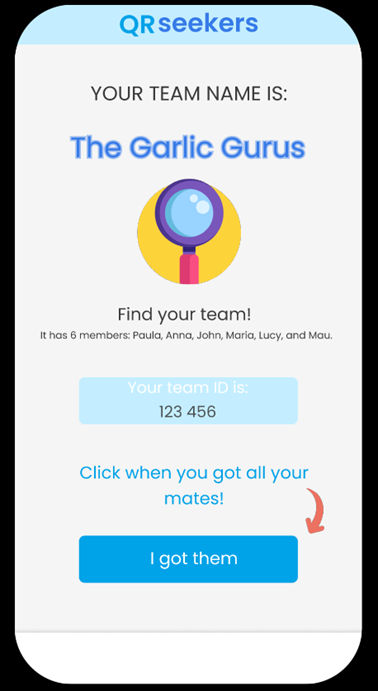
\includegraphics[width=0.4\textwidth]{figure6.png}
\caption{Team screen.}
\label{fig:1}
\end{figure}

\subsection{Pantalla de espera para el inicio del juego}

\begin{itemize}
    \item Tiempo de inicio del juego: Se indica una hora estimada para el comienzo del juego (en este caso, alrededor de las 13:00 h), y se muestra un ícono de reloj que refuerza la idea de la espera.
    \item Reglas del juego: Nuevamente, las reglas se presentan para que los jugadores las tengan claras antes de empezar. Esto asegura que todos los participantes estén familiarizados con las normas del juego.
\end{itemize}

\begin{figure}[H]
\centering
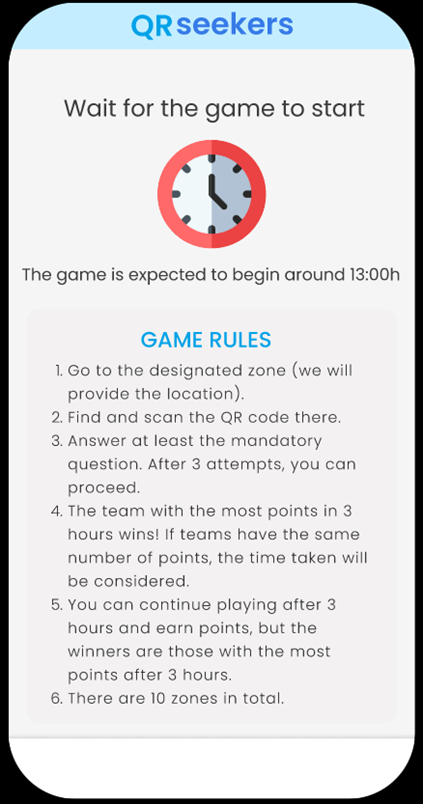
\includegraphics[width=0.4\textwidth]{figure7.png}
\caption{Waiting for the game to start screen.}
\label{fig:1}
\end{figure}

\subsection{Pantalla de ubicación}

\begin{itemize}
    \item Próxima ubicación: Esta pantalla muestra la siguiente ubicación a la que los jugadores deben dirigirse. En este ejemplo, se les indica que vayan a The Cathedral of Santa Ana.
    \item Pista: Se proporciona una pista que ayuda a encontrar el código QR, en este caso, se menciona que está 'Near the bus stop'.
    \item Acción a seguir: Hay una indicación clara para que los jugadores hagan clic en el ícono del mapa, lo que probablemente les dará la opción de abrir la ubicación en una aplicación de mapas. Además, una vez en la ubicación, se les pide que usen el ícono del escáner para encontrar el código QR.
\end{itemize}

\begin{figure}[H]
\centering
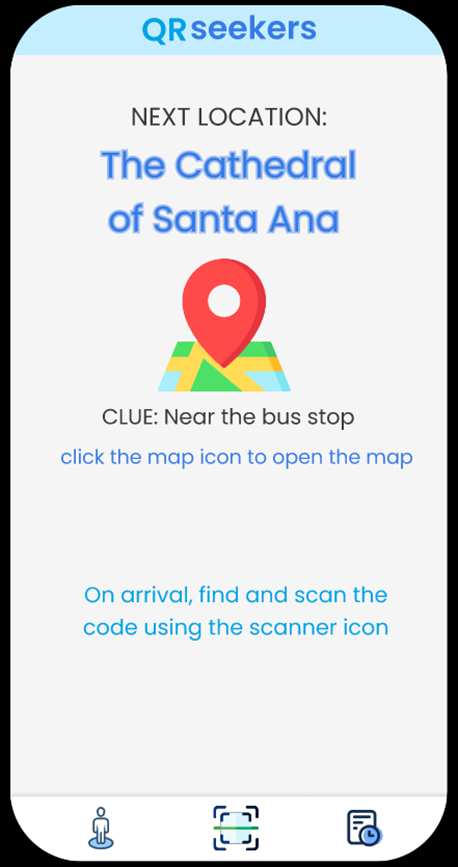
\includegraphics[width=0.4\textwidth]{figure8.png}
\caption{Location screen.}
\label{fig:1}
\end{figure}

\subsection{Pantalla de escaneo}

\begin{itemize}
    \item Escaneo del código: Esta pantalla es clave en la mecánica del juego, ya que permite a los usuarios escanear el código QR correspondiente a una ubicación específica. El diseño centraliza un ícono de escaneo que indica claramente al usuario que debe utilizar su cámara para capturar el código.
    \item Escribir el código: También se incluye la opción de escribir manualmente el código, lo que es útil en caso de que el escaneo no funcione.
    \item Ayuda: En caso de problemas para encontrar el código QR, se proporciona un número de WhatsApp para que los jugadores puedan pedir asistencia.
    \item Botón 'Next Zone': Una vez que el código QR ha sido escaneado correctamente o introducido manualmente, los jugadores pueden avanzar a la siguiente zona usando este botón.
\end{itemize}

\begin{figure}[H]
\centering
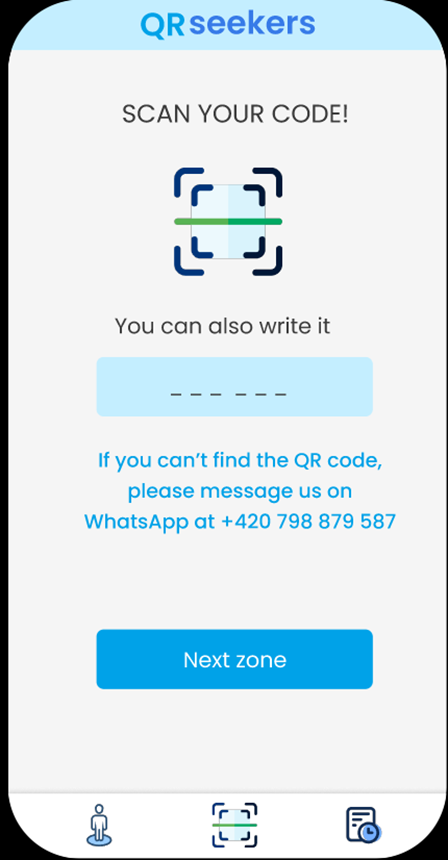
\includegraphics[width=0.4\textwidth]{figure9.png}
\caption{QR screen.}
\label{fig:1}
\end{figure}

\subsection{Pantalla de preguntas}

\begin{itemize}
    \item Pregunta obligatoria: Aquí se plantea una pregunta obligatoria relacionada con la ubicación que acaban de descubrir. En el ejemplo, la pregunta está relacionada con los relieves en el altar de la Catedral de Santa Ana. Este paso es necesario para poder avanzar en el juego.
    \item Preguntas opcionales: Además de la pregunta obligatoria, los usuarios tienen la opción de responder preguntas adicionales para ganar puntos extra, lo que añade una dimensión competitiva. En este caso, se pregunta sobre el inicio de la construcción de la catedral.
    \item Selección de respuestas: Se muestra un diseño de selección de respuestas tipo multiple choice (preguntas de opción múltiple), que simplifica la interacción y permite avanzar rápidamente.
\end{itemize}

\begin{figure}[H]
\centering
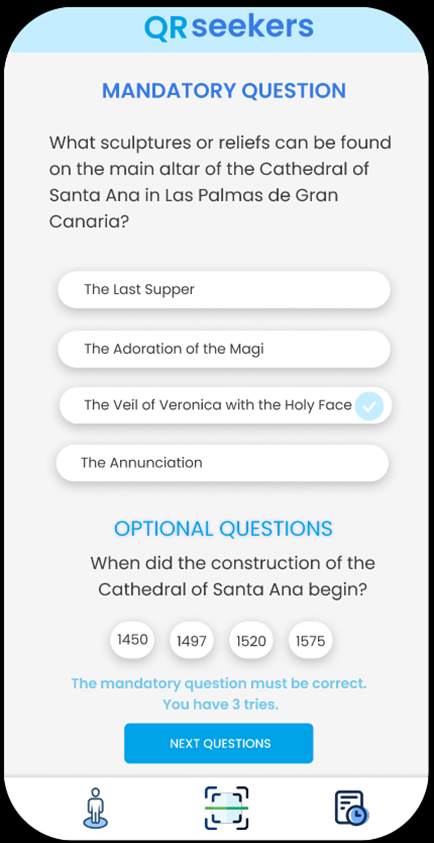
\includegraphics[width=0.4\textwidth]{figure10.png}
\caption{Questions screen.}
\label{fig:1}
\end{figure}

\subsection{Pantalla de final del juego}

\begin{itemize}
    \item Felicitaciones: Esta pantalla aparece una vez que el juego ha terminado, indicando que el jugador ha ganado una cantidad de puntos específica (en este caso, 60 puntos).
    \item Anuncio de ganadores: Se indica la hora a la que se anunciarán los ganadores y la ubicación en la que se hará dicho anuncio.
    \item Enlaces para resultados: Se incluye un enlace donde los jugadores pueden consultar la tabla de posiciones a través del sitio web de QRseekers.
    \item Opciones para continuar o terminar: Los jugadores pueden elegir si desean seguir jugando (si el juego permite más zonas) o finalizar su participación haciendo clic en 'I am done'.
\end{itemize}

\begin{figure}[H]
\centering
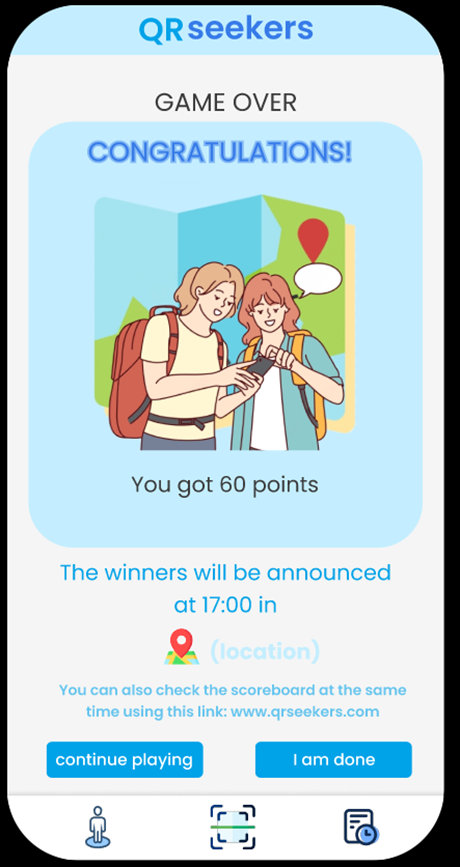
\includegraphics[width=0.4\textwidth]{figure11.png}
\caption{End screen.}
\label{fig:1}
\end{figure}

\subsection{Pantalla de recuperación de contraseña}

\begin{itemize}
    \item Solicitud de restablecimiento de contraseña: Esta pantalla permite a los usuarios recuperar su contraseña ingresando su correo electrónico. Un enlace de restablecimiento será enviado a su dirección.
    \item Diseño sencillo: El diseño es minimalista, lo que facilita la interacción rápida y directa para aquellos que necesiten recuperar su cuenta.
\end{itemize}

\begin{figure}[H]
\centering
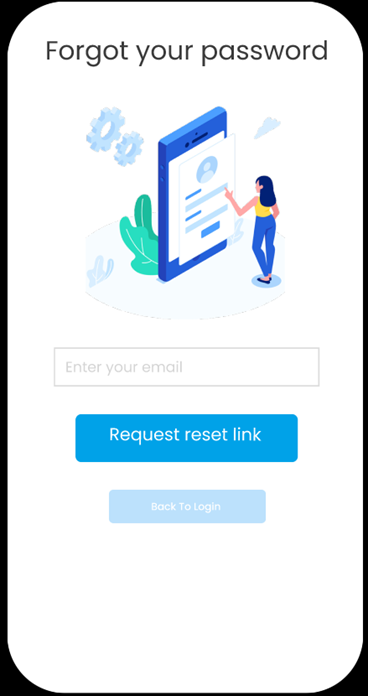
\includegraphics[width=0.4\textwidth]{figure12.png}
\caption{Forgot password screen.}
\label{fig:1}
\end{figure}

\subsection{Pantalla de restablecimiento de contraseña}

\begin{itemize}
    \item Creación de nueva contraseña: En esta pantalla, los usuarios pueden ingresar una nueva contraseña y confirmarla para completar el proceso de restablecimiento.
    \item Botón de confirmación: El botón 'Submit selection' permite confirmar.
\end{itemize}

\begin{figure}[H]
\centering
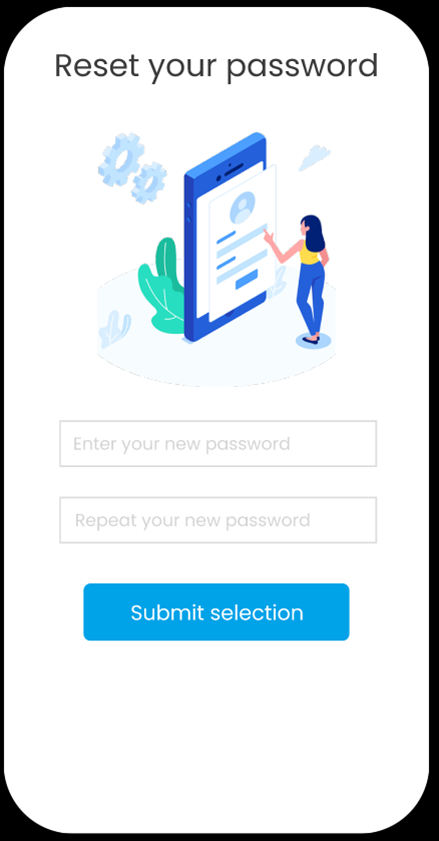
\includegraphics[width=0.4\textwidth]{figure13.png}
\caption{Forgot password screen.}
\label{fig:1}
\end{figure}

\subsection{Pantalla de información del usuario}

\begin{itemize}
    \item Avatar del usuario: En la parte superior, hay un ícono personalizado que representa al usuario, en este caso, una ilustración de un zorro. Esto puede haber sido seleccionado previamente por el usuario como avatar.
    \item Información personal: nombre personal, nombre de usuario, correo electrónico, equipo actual, opciones de edición, cambio de contraseña.
\end{itemize}

\begin{figure}[H]
\centering
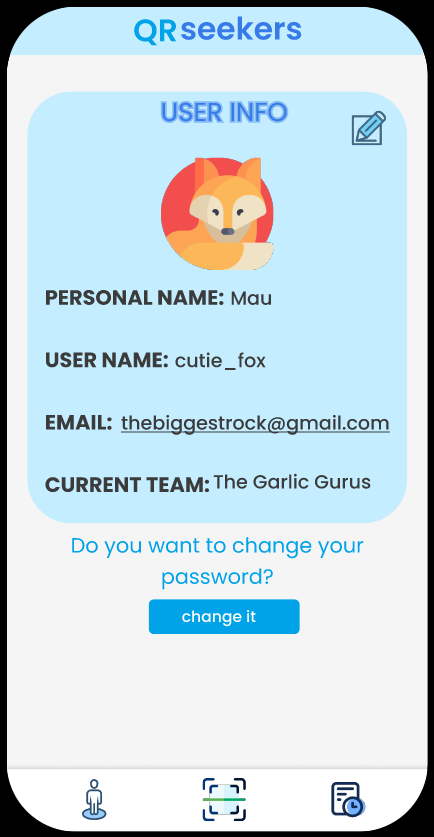
\includegraphics[width=0.4\textwidth]{figure14.png}
\caption{User info screen.}
\label{fig:1}
\end{figure}

\newpage

\section{Aspectos generales de diseño}
Llegados a este punto, podemos decir que cada pantalla mantiene un diseño coherente, siguiendo una línea gráfica consistente con el uso de colores y tipografías que reflejan la identidad de QRseekers, ayudando a crear una experiencia de usuario unificada. 

Además de esto, la disposición de la información es clara y concisa, lo que hace que la navegación entre las diferentes pantallas sea intuitiva. También observamos que la información está estructurada de manera clara, asegurando que los usuarios sepan qué pasos tomar a continuación en cada etapa del juego.

Así mismo, las pantallas están diseñadas para promover el trabajo en equipo, brindando información que resalta la importancia de la cooperación entre los miembros.

\newpage

\section{Conclusión}
El futuro de QRseekers es prometedor, ya que su diseño modular permite agregar fácilmente nuevas funcionalidades y juegos. A medida que más ciudades se sumen, la aplicación podrá ofrecer nuevas dinámicas, como eventos en vivo o colaboraciones con museos e instituciones culturales. Con el potencial de convertirse en una plataforma líder en el ámbito de los juegos urbanos y el turismo interactivo, QRseekers se perfila como una herramienta innovadora para quienes buscan explorar de una manera diferente y educativa.

\newpage
\hspace{0pt} %

\end{document}